% $Id$

\subsection{\label{ssec:high-arch}High-level, proposed \emph{vic} Architecture}

We have drawn a high-level overview of the proposed \emph{vic} architecture
(sender only) that has congestion control modules as in
Figure~\ref{fig:high-vic-arch}.  This figure represents a high-level overview of
\emph{vic} so that we could see the major components of the system, and how they
are interacting with each other. 

\vspace{1cm}

\begin{figure}[!h]
\begin{center}
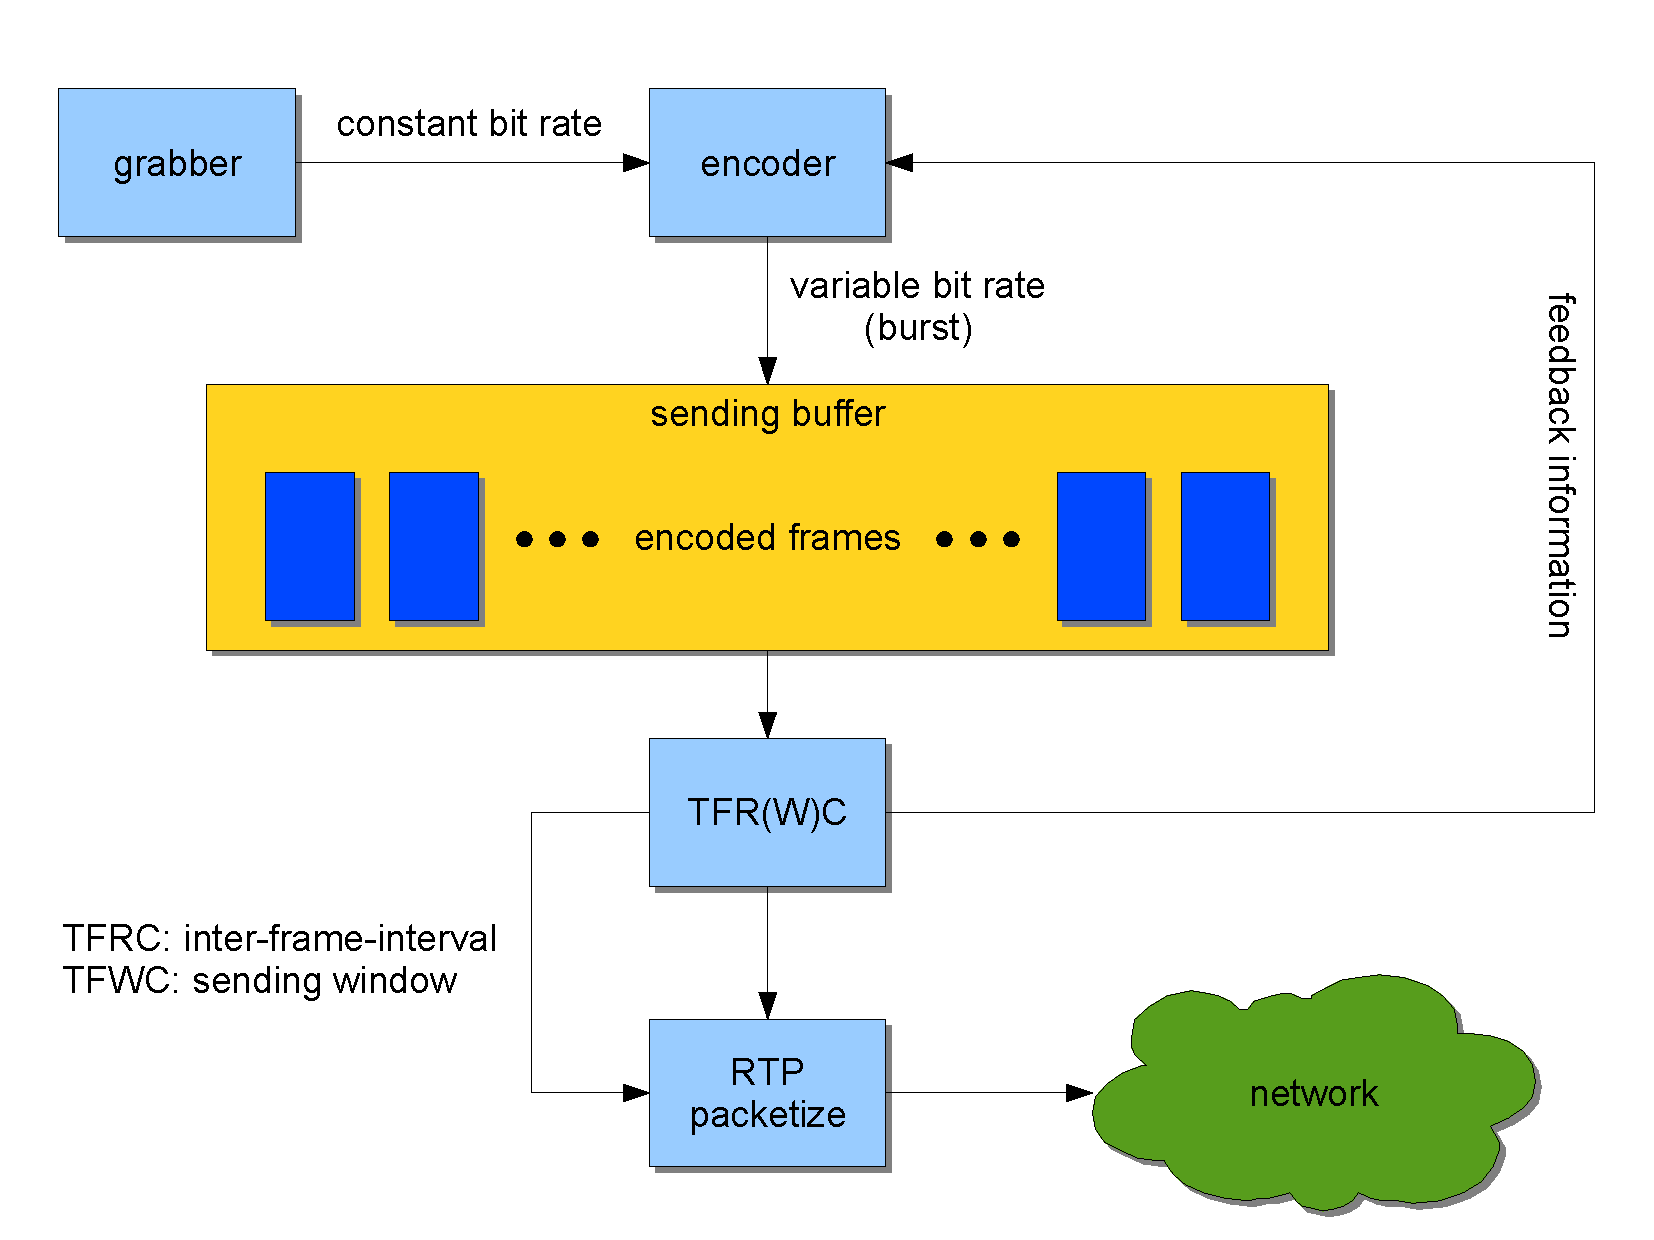
\includegraphics[scale=.5]{./img/high-vic-arch}
\caption{\label{fig:high-vic-arch}High-level, proposed \emph{vic} Architecture 
with CC Mechanisms}
\end{center}
\end{figure}

Unlike to the sender, we envisage the architecture of the receiver is relatively
simple. For example, upon a packet reception, it will be inserted to a receive
buffer, subsequently decoded (and some color conversion if necessary), and
finally displayed in a output device. Depending upon a codec, the rendered
frames may not be discarded immediately, but will be kept for some times before
they get purged.

\subsection{\label{ssec:vic-overview}\emph{vic} Overview by Example}

In this subsection, we describe how \emph{vic} works. To do so, we take the
still grabber (\texttt{grabber-still.cpp}) as an example and describe how
packets are transmitted.  The purpose of this analysis is to figure out how
\emph{vic} works and, from that, we would like to know how to design the
congestion control APIs. The still grabber can be used when we want to feed
pre-recored video sequences to the \emph{vic} system\footnote{One should start
\emph{vic} using the following command: \texttt{./vic -XstillGrabber \emph{(IP
address)}/\emph{(port number)}}.}. Currently, the still grabber in \emph{vic}
can take a JPG image file (4:2:2) and a CIF formatted video file.
Figure~\ref{fig:still-grabber} shows a class-diagram like figure that how the
still grabber generates packets. \\

\begin{figure}[!h] 
\begin{center}
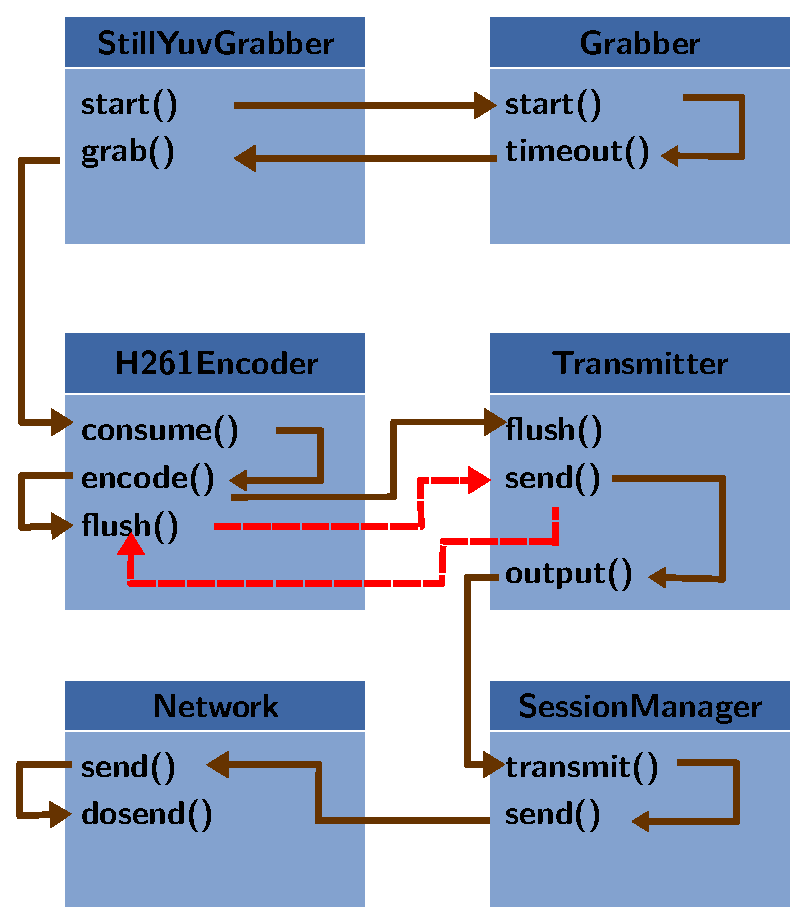
\includegraphics[scale=.5]{./img/still-grabber}
\caption{\label{fig:still-grabber}Still Grabber Information Flow}
\end{center} 
\end{figure}

Once the still device loads a file (either a JPG or a CIF file) into the memory,
it invokes \texttt{StillGrabber} or \texttt{StillYuvGrabber} depending upon a
file type. Assuming \texttt{StillYuvGrabber} is called, it sets the frame size
by calling \texttt{setsize()} method, and calls
\texttt{StillYuvGrabber::start()} which again calls \texttt{Grabber::start()}.
\texttt{Grabber::start()} basically sets the frame clock and timer using
\texttt{timeout()} method.  Then, \texttt{StillYuvGrabber::grab()} starts
grabbing video frames from the memory and passes to the encoder
(\texttt{encoder-h261.cpp}): in this case, \texttt{H261PixelEncoder::consume()}
will be called. After that, it starts encoding macro-blocks given a set of YUV
inputs and sends the encoded frames to the transmit module
(\texttt{SessionManager::transmit()}). The encoder provides the encoded frames
to the transmit module as long as they are available: see the dashed line in
Figure~\ref{fig:still-grabber}.  \texttt{SessionManager::transmit()} then
packetizes the frames and sends it to the network. \\

This is an example of how \emph{vic} takes input from a file, encodes the
frames, packetizes them, and sends them to the network. The core part of the
congestion control module could sit in between the codecs and the transmit
module. Instead of passing the encoded frames directly to the transmit module,
the encoded frames could be queued in some send buffer, and the congestion
control module picks up the frames determined by its suggested rate, for
example, if it is TFRC then it picks up the frames in a certain interval, or if
it is TFWC then it pick up the frames as long as the sending window allows. 

\newpage
